
\documentclass[letterpaper]{article}
%\usepackage{aaai}
\usepackage{times}
\usepackage{helvet}
\usepackage{algorithm}
\usepackage{algpseudocode}
\usepackage{courier}
\usepackage{graphicx}
\graphicspath{{./figure/}}
\frenchspacing
\setlength{\pdfpagewidth}{8.5in}
\setlength{\pdfpageheight}{11in}
\begin{document}    
\section{Efficient Matching by Movement Approximation}
\section{Tracking Objects with Common Movement}\label{trackingBySpatialReasoning}

One challenge is to determine a match between identical objects that are close to each other and have  similar trajectories.  

Figure \ref{SCOExample_2}.a  shows a scene where objects A and B form a slope and three identical squares, $o_1$, $o_2$ and $o_3$, are lying on the slope. Figure \ref{SCOExample_2}.b is a subsequent image where the three squares have rolled down slightly. There are 6 ways in total to match the squares in the two images but only $\{o_1 \sim o_4, o_2 \sim o_5, o_3 \sim o_6\}$ is possible. Because they do not use reasoning about the spatial relations between the squares, some optimization algorithms, e.g.\ minimizing centroid shift, will tend to match $o_2$ with $o_6$. In many cases, object dynamics, such as velocities, are unavailable, thus many of the state-of-the-art tracking algorithms will not work well because of the lack of a suitable dynamic model. 

Humans can solve this case efficiently using spatial reasoning. Since we know the objects are moving at a similar velocity, the relative spatial changes among them are subtle. Hence the spatial relations between those objects are unlikely to become inverted while they are moving. When matching, we try to keep the original spatial relations among the subsequent objects. 

We emulate this reasoning in testing a match by first identifying those objects that are following a similar trajectory and then determining whether any relation has become inverted in the subsequent image. 

Objects are likely to follow a common trajectory if they are all in contact with some other objects and the contact relations are the same. The objects may be influenced in the same way since their interactions are through the contacts with the other objects. We say that such objects form a \emph{spatially correlated object} (SCO). Figure \ref{SCOExample} shows some examples of SCOs in a typical Angry Birds scenario.

Given a set of initial objects, we obtain the SCOs by checking the node equivalence in the corresponding EGSR network. A node is equivalent to another if the two nodes have the same contact relations with other nodes. Thus the slope example has only one SCO: $\{o_1, o_2, o_3\}$ (see Figure \ref{SCOExample_2}.c).

Having identified an SCO, we then check the spatial relations between the matched objects in the subsequent image. Formally, let $R$ be a set of EGSR relations. The converse of a relation $r \in R$ is written as $r^{\prime} \in R$. Given a group objects that form a spatially correlated object in the initial image $O = \{o_1, o_2, ... , o_k\}$ and a set of subsequent objects $O^\prime = \{o^{\prime}_1, o^{\prime}_2, ..., o^{\prime}_k \}$ with a match, $\forall i\leq k, o_i \sim o^{\prime}_i$, between them, the spatial constraints can be written as $\forall o_i,o_j\in O, \exists r\in R$ such that $o_i \{r\} o_j \Rightarrow o^{\prime}_i \{r^{\prime}\} o^{\prime}_j$ \emph{does not hold}, for $i,j \leq k$. If a match violates the constraints, we will try all the other possible matches for the SCO until the violation is resolved. 

In the slope example, the match $\{o_1\sim o_4, o_3\sim o_5, o_2 \sim o_6\}$ violates the constraint because $o_2\{LEFT\}o_3$ and $o_6\{RIGHT\}o_5$ where $RIGHT$ is the converse of $LEFT$.

\begin{figure}[h!]
\centering\includegraphics[scale=0.7]{SCOScenario.png}\caption{(a) A typical Angry Birds scenario (b) SCOs (each highlighted by a different color)}
\label{SCOExample}
\end{figure}

\begin{figure}[h!]
\centering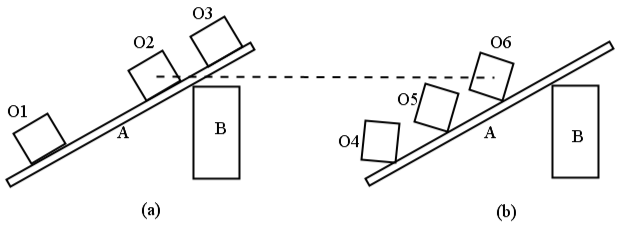
\includegraphics[scale=0.3]{SCOScenario_2.png}\caption{(a) An initial scene (b) A subsequent scene where the squares have rolled down slightly (c) The EGSR constraint network of the initial scene (only retain the edges indicating contacts) and the SCO}
\label{SCOExample_2}
\end{figure}

\end{document}